\documentclass[man,floatsintext]{apa6}
\usepackage{lmodern}
\usepackage{amssymb,amsmath}
\usepackage{ifxetex,ifluatex}
\usepackage{fixltx2e} % provides \textsubscript
\ifnum 0\ifxetex 1\fi\ifluatex 1\fi=0 % if pdftex
  \usepackage[T1]{fontenc}
  \usepackage[utf8]{inputenc}
\else % if luatex or xelatex
  \ifxetex
    \usepackage{mathspec}
  \else
    \usepackage{fontspec}
  \fi
  \defaultfontfeatures{Ligatures=TeX,Scale=MatchLowercase}
\fi
% use upquote if available, for straight quotes in verbatim environments
\IfFileExists{upquote.sty}{\usepackage{upquote}}{}
% use microtype if available
\IfFileExists{microtype.sty}{%
\usepackage{microtype}
\UseMicrotypeSet[protrusion]{basicmath} % disable protrusion for tt fonts
}{}
\usepackage{hyperref}
\hypersetup{unicode=true,
            pdftitle={A practical primer on processing semantic property norm data},
            pdfauthor={Erin M. Buchanan, Simon De Deyne, \& Maria Montefinese},
            pdfkeywords={semantic, property norm task, tutorial},
            pdfborder={0 0 0},
            breaklinks=true}
\urlstyle{same}  % don't use monospace font for urls
\usepackage{color}
\usepackage{fancyvrb}
\newcommand{\VerbBar}{|}
\newcommand{\VERB}{\Verb[commandchars=\\\{\}]}
\DefineVerbatimEnvironment{Highlighting}{Verbatim}{commandchars=\\\{\}}
% Add ',fontsize=\small' for more characters per line
\usepackage{framed}
\definecolor{shadecolor}{RGB}{248,248,248}
\newenvironment{Shaded}{\begin{snugshade}}{\end{snugshade}}
\newcommand{\AlertTok}[1]{\textcolor[rgb]{0.94,0.16,0.16}{#1}}
\newcommand{\AnnotationTok}[1]{\textcolor[rgb]{0.56,0.35,0.01}{\textbf{\textit{#1}}}}
\newcommand{\AttributeTok}[1]{\textcolor[rgb]{0.77,0.63,0.00}{#1}}
\newcommand{\BaseNTok}[1]{\textcolor[rgb]{0.00,0.00,0.81}{#1}}
\newcommand{\BuiltInTok}[1]{#1}
\newcommand{\CharTok}[1]{\textcolor[rgb]{0.31,0.60,0.02}{#1}}
\newcommand{\CommentTok}[1]{\textcolor[rgb]{0.56,0.35,0.01}{\textit{#1}}}
\newcommand{\CommentVarTok}[1]{\textcolor[rgb]{0.56,0.35,0.01}{\textbf{\textit{#1}}}}
\newcommand{\ConstantTok}[1]{\textcolor[rgb]{0.00,0.00,0.00}{#1}}
\newcommand{\ControlFlowTok}[1]{\textcolor[rgb]{0.13,0.29,0.53}{\textbf{#1}}}
\newcommand{\DataTypeTok}[1]{\textcolor[rgb]{0.13,0.29,0.53}{#1}}
\newcommand{\DecValTok}[1]{\textcolor[rgb]{0.00,0.00,0.81}{#1}}
\newcommand{\DocumentationTok}[1]{\textcolor[rgb]{0.56,0.35,0.01}{\textbf{\textit{#1}}}}
\newcommand{\ErrorTok}[1]{\textcolor[rgb]{0.64,0.00,0.00}{\textbf{#1}}}
\newcommand{\ExtensionTok}[1]{#1}
\newcommand{\FloatTok}[1]{\textcolor[rgb]{0.00,0.00,0.81}{#1}}
\newcommand{\FunctionTok}[1]{\textcolor[rgb]{0.00,0.00,0.00}{#1}}
\newcommand{\ImportTok}[1]{#1}
\newcommand{\InformationTok}[1]{\textcolor[rgb]{0.56,0.35,0.01}{\textbf{\textit{#1}}}}
\newcommand{\KeywordTok}[1]{\textcolor[rgb]{0.13,0.29,0.53}{\textbf{#1}}}
\newcommand{\NormalTok}[1]{#1}
\newcommand{\OperatorTok}[1]{\textcolor[rgb]{0.81,0.36,0.00}{\textbf{#1}}}
\newcommand{\OtherTok}[1]{\textcolor[rgb]{0.56,0.35,0.01}{#1}}
\newcommand{\PreprocessorTok}[1]{\textcolor[rgb]{0.56,0.35,0.01}{\textit{#1}}}
\newcommand{\RegionMarkerTok}[1]{#1}
\newcommand{\SpecialCharTok}[1]{\textcolor[rgb]{0.00,0.00,0.00}{#1}}
\newcommand{\SpecialStringTok}[1]{\textcolor[rgb]{0.31,0.60,0.02}{#1}}
\newcommand{\StringTok}[1]{\textcolor[rgb]{0.31,0.60,0.02}{#1}}
\newcommand{\VariableTok}[1]{\textcolor[rgb]{0.00,0.00,0.00}{#1}}
\newcommand{\VerbatimStringTok}[1]{\textcolor[rgb]{0.31,0.60,0.02}{#1}}
\newcommand{\WarningTok}[1]{\textcolor[rgb]{0.56,0.35,0.01}{\textbf{\textit{#1}}}}
\usepackage{graphicx,grffile}
\makeatletter
\def\maxwidth{\ifdim\Gin@nat@width>\linewidth\linewidth\else\Gin@nat@width\fi}
\def\maxheight{\ifdim\Gin@nat@height>\textheight\textheight\else\Gin@nat@height\fi}
\makeatother
% Scale images if necessary, so that they will not overflow the page
% margins by default, and it is still possible to overwrite the defaults
% using explicit options in \includegraphics[width, height, ...]{}
\setkeys{Gin}{width=\maxwidth,height=\maxheight,keepaspectratio}
\IfFileExists{parskip.sty}{%
\usepackage{parskip}
}{% else
\setlength{\parindent}{0pt}
\setlength{\parskip}{6pt plus 2pt minus 1pt}
}
\setlength{\emergencystretch}{3em}  % prevent overfull lines
\providecommand{\tightlist}{%
  \setlength{\itemsep}{0pt}\setlength{\parskip}{0pt}}
\setcounter{secnumdepth}{0}
% Redefines (sub)paragraphs to behave more like sections
\ifx\paragraph\undefined\else
\let\oldparagraph\paragraph
\renewcommand{\paragraph}[1]{\oldparagraph{#1}\mbox{}}
\fi
\ifx\subparagraph\undefined\else
\let\oldsubparagraph\subparagraph
\renewcommand{\subparagraph}[1]{\oldsubparagraph{#1}\mbox{}}
\fi

%%% Use protect on footnotes to avoid problems with footnotes in titles
\let\rmarkdownfootnote\footnote%
\def\footnote{\protect\rmarkdownfootnote}


  \title{A practical primer on processing semantic property norm data}
    \author{Erin M. Buchanan\textsuperscript{1}, Simon De Deyne\textsuperscript{2}, \& Maria Montefinese\textsuperscript{3}}
    \date{}
  
\shorttitle{Processing Norms}
\affiliation{
\vspace{0.5cm}
\textsuperscript{1} Harrisburg University of Science and Technology\\\textsuperscript{2} University of Melbourne\\\textsuperscript{3} University of Padua}
\keywords{semantic, property norm task, tutorial}
\usepackage{csquotes}
\usepackage{upgreek}
\captionsetup{font=singlespacing,justification=justified}

\usepackage{longtable}
\usepackage{lscape}
\usepackage{multirow}
\usepackage{tabularx}
\usepackage[flushleft]{threeparttable}
\usepackage{threeparttablex}

\newenvironment{lltable}{\begin{landscape}\begin{center}\begin{ThreePartTable}}{\end{ThreePartTable}\end{center}\end{landscape}}

\makeatletter
\newcommand\LastLTentrywidth{1em}
\newlength\longtablewidth
\setlength{\longtablewidth}{1in}
\newcommand{\getlongtablewidth}{\begingroup \ifcsname LT@\roman{LT@tables}\endcsname \global\longtablewidth=0pt \renewcommand{\LT@entry}[2]{\global\advance\longtablewidth by ##2\relax\gdef\LastLTentrywidth{##2}}\@nameuse{LT@\roman{LT@tables}} \fi \endgroup}


\usepackage{lineno}

\linenumbers

\authornote{Add complete departmental affiliations for each author here. Each new line herein must be indented, like this line.

Enter author note here.

Correspondence concerning this article should be addressed to Erin M. Buchanan, 326 Market St., Harrisburg, PA 17101. E-mail: \href{mailto:ebuchanan@harrisburgu.edu}{\nolinkurl{ebuchanan@harrisburgu.edu}}}

\abstract{
Semantic property listing tasks require participants to generate short propositions (e.g., \textless{}barks\textgreater{}, \textless{}has fur\textgreater{}) for a specific concept (e.g., dog). This task is the cornerstone of the creation of semantic property norms which are essential for modelling, stimuli creation, and understanding similarity between concepts. However, despite the wide applicability of semantic property norms for a large variety of concepts across different groups of people, the methodological aspects of the property listing task have received less attention, even though the procedure and processing of the data can substantially affect the nature and quality of the measures derived from them. The goal of this paper is to provide a practical primer on how to collect and process semantic property norms. We will discuss the key methods to elicit semantic properties and compare different methods to derive meaningful representations from them. This will cover the role of instructions and test context, property pre-processing (e.g., lemmatization), property weighting, and relationship encoding using ontologies. With these choices in mind, we propose and demonstrate a processing pipeline that transparently documents these steps resulting in improved comparability across different studies. The impact of these choices will be demonstrated using intrinsic (e.g.~reliability, number of properties) and extrinsic measures (e.g., categorization, semantic similarity, lexical processing). Example data and the impact of choice decisions will be provided. This practical primer will offer potential solutions to several longstanding problems and allow researchers to develop new property listing norms overcoming the constraints of previous studies.


}

\begin{document}
\maketitle

\begin{enumerate}
\def\labelenumi{\arabic{enumi}.}
\tightlist
\item
  Available feature norms and their format
\end{enumerate}

\begin{itemize}
\tightlist
\item
  Property listing task original work: ({\textbf{???}}); ({\textbf{???}}); ({\textbf{???}}); ({\textbf{???}})
\item
  English: ({\textbf{???}}), ({\textbf{???}}), ({\textbf{???}}), ({\textbf{???}}), ({\textbf{???}})
\item
  Italian: ({\textbf{???}}); ({\textbf{???}}), ({\textbf{???}})
\item
  German: ({\textbf{???}})
\item
  Portuguese: ({\textbf{???}})
\item
  Spanish: ({\textbf{???}})
\item
  Dutch: ({\textbf{???}})
\item
  Blind participants: ({\textbf{???}})
\end{itemize}

I'm sure there are more, here's what we cited recently.

Define concept, feature for clarity throughout - make sure you use these two terms consistently.

\begin{enumerate}
\def\labelenumi{\arabic{enumi}.}
\setcounter{enumi}{1}
\tightlist
\item
  Pointers about how to collect the data
\end{enumerate}

\begin{enumerate}
\def\labelenumi{\alph{enumi}.}
\tightlist
\item
  instructions, generation, verification, importance
\end{enumerate}

I really like the way the CSLB did it: \url{https://cslb.psychol.cam.ac.uk/propnorms}

They showed the concept, then had a drop down menu for is/has/does, and then the participant typed in a final window. That type of system would solve about half the problems I am going to describe below about using multi-word sequences. Might be some other suggestions, but for that type of processing, you could do combinations and have more consistent data easily.

\begin{enumerate}
\def\labelenumi{\arabic{enumi}.}
\setcounter{enumi}{2}
\tightlist
\item
  Typical operations performed on features
\end{enumerate}

\begin{figure}
\centering
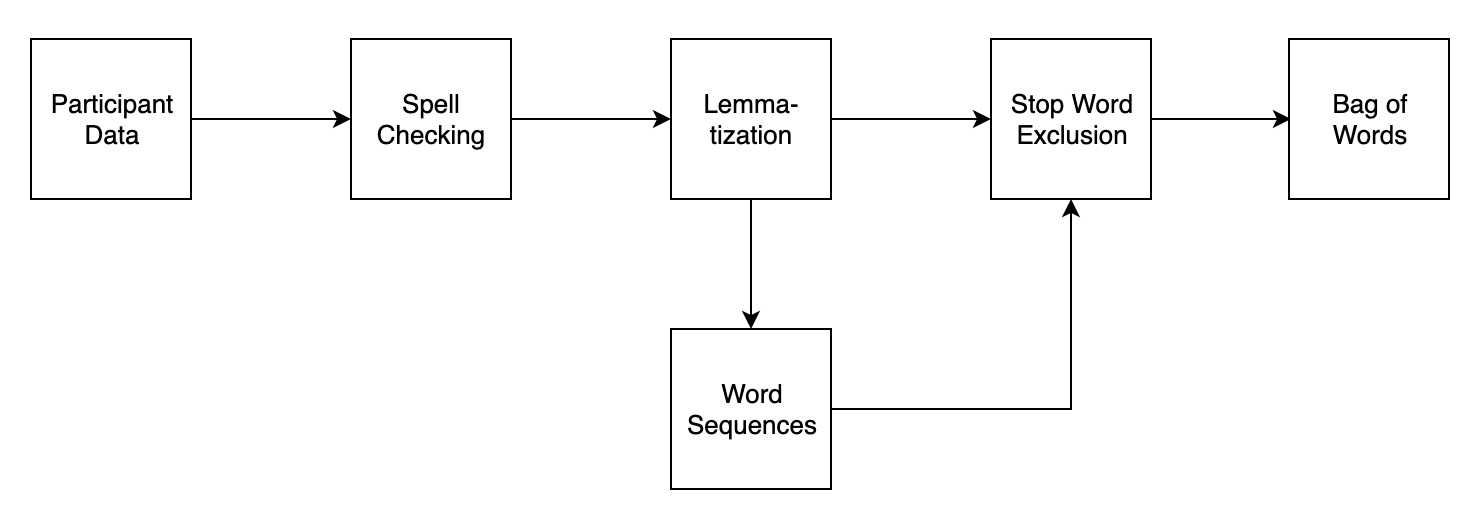
\includegraphics{flow_chart.png}
\caption{(\#fig:flow\_chart)Flow chart of proposed semantic processing feature steps.}
\end{figure}

In the next several sections, we provide a tutorial using \emph{R} on how data from the semantic property norm task might be processed from raw input to finalized output. Figure @ref(fig:flow\_chart) portrays the proposed set of steps including spell checking, lemmatization, exclusion of stop words, and final processing in a multi-word sequence approach or a bag of words approach. After detailing these steps, the final data form will compared to previous norms to determine the usefulness of this approach.

\hypertarget{materials-and-data-format}{%
\subsection{Materials and Data Format}\label{materials-and-data-format}}

The data for this tutorial includes 9553 unique concept-feature responses for 104 concepts from ({\textbf{???}}) that were included in ({\textbf{???}}), ({\textbf{???}}), and ({\textbf{???}}). The data should be structured in tidy format wherein each concept-feature observation is a row and each column is a variable ({\textbf{???}}). Therefore, the data includes a \texttt{word} column with the normed concept and an \texttt{answer} column with the participant answer.

\begin{table}[H]
\centering\begin{table}[H]
\centering
\begin{tabular}{l>{\raggedright\arraybackslash}p{30em}}
\toprule
word & answer\\
\midrule
airplane & you fly in it  its big  it is fast  they are expensive  they are at an airport  you have to be trained to fly it  there are lots of seats  they get very high up\\
airplane & wings engine pilot cockpit tail\\
airplane & wings  it flys  modern technology  has passengers  requires a pilot  can be dangerous  runs on gas  used for travel\\
airplane & wings  flys  pilot  cockpit  uses gas  faster travel\\
airplane & wings  engines  passengers  pilot(s)  vary in size and color\\
\addlinespace
airplane & wings  body  flies  travel\\
\bottomrule
\end{tabular}
\end{table}
\end{table}

This data was collected using the instructions provided by ({\textbf{???}}), however, in contrast to the suggestions for consistency detailed above ({\textbf{???}}), each participant was simply given a large text box to include their answer. Each answer includes multiple embedded features, and the tutorial proceeds to demonstrate potential processing addressing the data in this nature. With structured data entry for participants, the suggested processing steps are reduced.

\hypertarget{spelling}{%
\subsection{Spelling}\label{spelling}}

Spell checking can be automated with the \texttt{hunspell} package in \emph{R} ({\textbf{???}}), which is the spell checking library used in popular programs such as FireFox, Chrome, RStudio, and OpenOffice. Each \texttt{answer} can be checked for misspellings across an entire column of answers, which is located in the \texttt{master} dataset. The default dictionary is American English, and the \texttt{hunspell} vignettes provide details on how to import your own dictionary for non-English languages. The choice of dictionary should also normalize between multiple varieties of the same language, for example, the \texttt{"en\_GB"} would convert to British English spellings.

\scriptsize

\begin{Shaded}
\begin{Highlighting}[]
\CommentTok{## Install the hunspell package if necessary}
\CommentTok{#install.packages("hunspell")}
\KeywordTok{library}\NormalTok{(hunspell)}
\CommentTok{## Check the participant answers}
\CommentTok{## The output is a list of spelling errors for each line}
\NormalTok{spelling_errors <-}\StringTok{ }\KeywordTok{hunspell}\NormalTok{(master}\OperatorTok{$}\NormalTok{answer, }\DataTypeTok{dict =} \KeywordTok{dictionary}\NormalTok{(}\StringTok{"en_US"}\NormalTok{))}
\end{Highlighting}
\end{Shaded}

\normalsize

The result from the \texttt{hunspell()} function is a list object of spelling errors for each row of data. For example, when responding to \emph{apple}, a participant wrote \emph{fruit grocery store orchard red green yelloe good with peanut butter good with caramell}, and the spelling errors were denoted as \emph{yelloe caramell}. After checking for errors, the \texttt{hunspell\_suggest()} function was used to determine the most likely replacement for each error.

\begin{Shaded}
\begin{Highlighting}[]
\CommentTok{## Check for suggestions}
\NormalTok{spelling_suggest <-}\StringTok{ }\KeywordTok{lapply}\NormalTok{(spelling_errors, hunspell_suggest)}
\end{Highlighting}
\end{Shaded}

For \emph{yelloe}, both \emph{yellow yell} were suggested, and \emph{caramel caramels caramel l camellia camel} were suggested for \emph{caramell}. The suggestions are presented in most probable order, and using a few loops with the substitute (\texttt{gsub}) function, we can replace all errors with the most likely replacement in a new dataset \texttt{spell\_checked}. A specialized dictionary with precoded error responses and corrections could be implemented at this stage. Other paid alternatives, such as Bing Spell Check, can be a useful avenue for datasets that may contain brand names (i.e, \emph{apple} versus \emph{Apple}) or slang terms.

\begin{Shaded}
\begin{Highlighting}[]
\CommentTok{## Replace with most likely suggestion}
\NormalTok{spell_checked <-}\StringTok{ }\NormalTok{master}
\CommentTok{### Loop over the data.frame}
\ControlFlowTok{for}\NormalTok{ (i }\ControlFlowTok{in} \DecValTok{1}\OperatorTok{:}\KeywordTok{nrow}\NormalTok{(spell_checked))\{}
  \CommentTok{### See if there are spelling errors}
  \ControlFlowTok{if}\NormalTok{ (}\KeywordTok{length}\NormalTok{(spelling_errors[[i]]) }\OperatorTok{>}\StringTok{ }\DecValTok{0}\NormalTok{) \{}
    \CommentTok{### Loop over all errors}
    \ControlFlowTok{for}\NormalTok{ (q }\ControlFlowTok{in} \DecValTok{1}\OperatorTok{:}\KeywordTok{length}\NormalTok{(spelling_errors[[i]]))\{}
      \CommentTok{### Replace with the first answer}
\NormalTok{      spell_checked}\OperatorTok{$}\NormalTok{answer[i] <-}\StringTok{ }\KeywordTok{gsub}\NormalTok{(spelling_errors[[i]][q], }
\NormalTok{                                      spelling_suggest[[i]][[q]][}\DecValTok{1}\NormalTok{],}
\NormalTok{                                      spell_checked}\OperatorTok{$}\NormalTok{answer[i])}
\NormalTok{    \}}
\NormalTok{  \}}
\NormalTok{\}}
\end{Highlighting}
\end{Shaded}

\hypertarget{lemmatization}{%
\subsection{Lemmatization}\label{lemmatization}}

The next step approaches the clustering of word forms into their lemma or head word from a dictionary. The process of lemmatizing words involves using a lexeme set (i.e., all words forms that have the same meaning, \emph{am, are, is}) to convert into a common lemma (i.e., \emph{be}) from a trained dictionary. In contrast, stemming involves processing words using heuristics to remove affixes or inflections, such as \emph{ing} or \emph{s}. The stem or root word may not reflect an actual word in the langauge, as simply removing an affix does not necessarily produce the lemma. For example, in response to \emph{airplane}, \emph{flying} can be easily converted to \emph{fly} by removing the \emph{ing} inflection. However, this same heuristic converts the feature \emph{wings} into \emph{w} after removing both the \emph{s} for a plural marker and the \emph{ing} participle marker. Several packages for \emph{R} include customizable stemmers, notably the \texttt{hunspell}, \texttt{corpus} ({\textbf{???}}), and \texttt{tm} ({\textbf{???}}) packages.

Lemmatization is the likely choice for processing property norms, and this process can be achieved by installing \texttt{TreeTagger} ({\textbf{???}}) and the \texttt{koRpus} package in \emph{R} ({\textbf{???}}). TreeTagger is a trained tagger designed to annotate part of speech and lemma information in text, and parameter files are available for multiple langauges. The koRpus package includes functionality to use TreeTagger in \emph{R}. After installing the package and TreeTagger, we will create a unique set of tokenized words to lemmatize to speed computation.

\begin{Shaded}
\begin{Highlighting}[]
\NormalTok{lemmas <-}\StringTok{ }\NormalTok{spell_checked}
\CommentTok{## Install the koRpus package}
\CommentTok{#install.packages("koRpus")}
\CommentTok{#install.packages("koRpus.lang.en")}
\CommentTok{## You must load both packages separately}
\KeywordTok{library}\NormalTok{(koRpus)}
\KeywordTok{library}\NormalTok{(koRpus.lang.en)}
\CommentTok{## Install TreeTagger }
\CommentTok{#https://www.cis.uni-muenchen.de/~schmid/tools/TreeTagger/}
\CommentTok{## Find all types for faster lookup}
\NormalTok{all_answers <-}\StringTok{ }\KeywordTok{tokenize}\NormalTok{(lemmas}\OperatorTok{$}\NormalTok{answer, }\DataTypeTok{format =} \StringTok{"obj"}\NormalTok{, }\DataTypeTok{tag =}\NormalTok{ F)}
\NormalTok{all_answers <-}\StringTok{ }\KeywordTok{unique}\NormalTok{(all_answers)}
\end{Highlighting}
\end{Shaded}

The \texttt{treetag()} function calls the installation of TreeTagger to provide part of speech tags and lemmas for each token. Importantly, the \texttt{path} option should be the directory of the TreeTagger installation.

\begin{Shaded}
\begin{Highlighting}[]
\CommentTok{## This function has both suppressWarnings & suppressMessages}
\CommentTok{## You should first view these to ensure proper processing}
\NormalTok{temp_tag <-}\StringTok{ }\KeywordTok{suppressWarnings}\NormalTok{(}
  \KeywordTok{suppressMessages}\NormalTok{(}
    \CommentTok{## Note: the NULL option is to control for the <unknown> that appears}
    \CommentTok{## to occur with the last word in each text}
    \KeywordTok{treetag}\NormalTok{(}\KeywordTok{c}\NormalTok{(all_answers, }\StringTok{"NULL"}\NormalTok{), }
            \CommentTok{## Control the parameters of treetagger}
            \DataTypeTok{treetagger=}\StringTok{"manual"}\NormalTok{, }\DataTypeTok{format=}\StringTok{"obj"}\NormalTok{,}
            \DataTypeTok{TT.tknz=}\OtherTok{FALSE}\NormalTok{, }\DataTypeTok{lang=}\StringTok{"en"}\NormalTok{,}
            \DataTypeTok{TT.options=}\KeywordTok{list}\NormalTok{(}\DataTypeTok{path=}\StringTok{"~/TreeTagger"}\NormalTok{, }\DataTypeTok{preset=}\StringTok{"en"}\NormalTok{))))}
\end{Highlighting}
\end{Shaded}

This function returns a tagged corpus object, which can be converted into a dataframe of the token-lemma information. The goal would be to replace inflected words with their lemmas, and therefore, unknown values, number tags, and equivalent values are ignored by subseting out these from the dataset.

\begin{Shaded}
\begin{Highlighting}[]
\CommentTok{## Remove all tags not using}
\NormalTok{replacement_lemmas <-}\StringTok{ }\NormalTok{temp_tag}\OperatorTok{@}\NormalTok{TT.res}
\NormalTok{replacement_lemmas <-}\StringTok{ }\KeywordTok{subset}\NormalTok{(replacement_lemmas, }
                             \CommentTok{#ignore punctuation}
\NormalTok{                             wclass }\OperatorTok{!=}\StringTok{ "punctuation"} \OperatorTok{&}
\StringTok{                             }\CommentTok{#unknown values}
\StringTok{                             }\NormalTok{lemma }\OperatorTok{!=}\StringTok{ "<unknown>"} \OperatorTok{&}\StringTok{ }
\StringTok{                             }\CommentTok{#numbers}
\StringTok{                             }\NormalTok{lemma}\OperatorTok{!=}\StringTok{ "@card@"} \OperatorTok{&}\StringTok{ }
\StringTok{                             }\CommentTok{#token should change more than case}
\StringTok{                             }\KeywordTok{tolower}\NormalTok{(token) }\OperatorTok{!=}\StringTok{ }\KeywordTok{tolower}\NormalTok{(lemma)) }
\end{Highlighting}
\end{Shaded}

\begin{table}[H]
\centering
\begin{tabular}{lllrl}
\toprule
token & tag & lemma & lttr & wclass\\
\midrule
is & VBZ & be & 2 & verb\\
are & VBP & be & 3 & verb\\
trained & VBN & train & 7 & verb\\
lots & NNS & lot & 4 & noun\\
seats & NNS & seat & 5 & noun\\
\addlinespace
wings & NNS & wing & 5 & noun\\
\bottomrule
\end{tabular}
\end{table}

From this dataset, you can use the \texttt{stringi} package ({\textbf{???}}) to replace all of the original tokens with their lemmas. This package allows for replacement lookup across a large set of subsitutions.

\begin{Shaded}
\begin{Highlighting}[]
\CommentTok{## Install the stringi package}
\CommentTok{#install.packages("stringi")}
\KeywordTok{library}\NormalTok{(stringi)}
\CommentTok{## Replace all the original tokens with new lemmas using \textbackslash{}\textbackslash{}b for word boundaries}
\NormalTok{lemmas}\OperatorTok{$}\NormalTok{answer <-}\StringTok{ }\KeywordTok{stri_replace_all_regex}\NormalTok{(}\DataTypeTok{str =}\NormalTok{ lemmas}\OperatorTok{$}\NormalTok{answer, }
                       \DataTypeTok{pattern =} \KeywordTok{paste}\NormalTok{(}\StringTok{"}\CharTok{\textbackslash{}\textbackslash{}}\StringTok{b"}\NormalTok{, replacement_lemmas}\OperatorTok{$}\NormalTok{token, }\StringTok{"}\CharTok{\textbackslash{}\textbackslash{}}\StringTok{b"}\NormalTok{, }\DataTypeTok{sep =} \StringTok{""}\NormalTok{),}
                       \DataTypeTok{replacement =}\NormalTok{ replacement_lemmas}\OperatorTok{$}\NormalTok{lemma,}
                       \DataTypeTok{vectorize_all =}\NormalTok{ F, }\KeywordTok{list}\NormalTok{(}\DataTypeTok{case_insensitive =} \OtherTok{TRUE}\NormalTok{))}
\end{Highlighting}
\end{Shaded}

\begin{table}[H]
\centering\begin{table}[H]
\centering
\begin{tabular}{l>{\raggedright\arraybackslash}p{30em}}
\toprule
word & answer\\
\midrule
airplane & you fly in it  its big  it be fast  they be expensive  they be at an airport  you have to be train to fly it  there be lot of seat  they get very high up\\
airplane & wing engine pilot cockpit tail\\
airplane & wing  it fly  modern technology  have passenger  require a pilot  can be dangerous  run on gas  use for travel\\
airplane & wing  fly  pilot  cockpit  use gas  fast travel\\
airplane & wing  engine  passenger  pilot(s)  vary in size and color\\
\addlinespace
airplane & wing  body  fly  travel\\
\bottomrule
\end{tabular}
\end{table}
\end{table}

\hypertarget{word-sequences}{%
\subsection{Word Sequences}\label{word-sequences}}

Multi-word sequences are often coded to mimic a ({\textbf{???}}) style model, with \enquote{is-a} and \enquote{has-a} type markers. If data were collected to include these markers, this step would be pre-encoded into the output data, rendering the following code unnecessary. A potential solution for processing messy data could be to search for specific part of speech sequences that mimic the \enquote{is-a} and \enquote{has-a} strings. An examination of the coding in ({\textbf{???}}) and ({\textbf{???}}) indicates that the feature tags are often verb-noun or verb-adjective-noun sequences. Using TreeTagger on each concept's answer set, we can obtain the parts of speech in context for each lemma. With \texttt{dplyr} ({\textbf{???}}), new columns are added to tagged data to show all bigram and trigram sequences. All verb-noun and verb-adjective-noun combinations are selected, and any words not part of these multi-word sequences are treated as unigrams. Finally, the \texttt{table()} function is used to tabulate the final count of n-grams and their frequency.

\begin{Shaded}
\begin{Highlighting}[]
\NormalTok{multi_words <-}\StringTok{ }\KeywordTok{data.frame}\NormalTok{(}\DataTypeTok{Word=}\KeywordTok{character}\NormalTok{(),}
                        \DataTypeTok{Feature=}\KeywordTok{character}\NormalTok{(), }
                        \DataTypeTok{Frequency=}\KeywordTok{numeric}\NormalTok{(), }
                        \DataTypeTok{stringsAsFactors=}\OtherTok{FALSE}\NormalTok{) }
\NormalTok{unique_concepts <-}\StringTok{ }\KeywordTok{unique}\NormalTok{(lemmas}\OperatorTok{$}\NormalTok{word)}
\CommentTok{## Install dplyr}
\CommentTok{#install.packages("dplyr")}
\KeywordTok{library}\NormalTok{(dplyr)}
\CommentTok{## Loop over each word}
\ControlFlowTok{for}\NormalTok{ (i }\ControlFlowTok{in} \DecValTok{1}\OperatorTok{:}\KeywordTok{length}\NormalTok{(unique_concepts))\{}
  \CommentTok{## Create parts of speech for clustering together}
\NormalTok{  temp_tag <-}\StringTok{ }\KeywordTok{suppressWarnings}\NormalTok{(}
    \KeywordTok{suppressMessages}\NormalTok{(}
      \KeywordTok{treetag}\NormalTok{(}\KeywordTok{c}\NormalTok{(lemmas}\OperatorTok{$}\NormalTok{answer[lemmas}\OperatorTok{$}\NormalTok{word  }\OperatorTok{==}\StringTok{ }\NormalTok{unique_concepts[i]], }\StringTok{"NULL"}\NormalTok{), }
          \CommentTok{## Control the parameters of treetagger}
          \DataTypeTok{treetagger=}\StringTok{"manual"}\NormalTok{, }\DataTypeTok{format=}\StringTok{"obj"}\NormalTok{,}
          \DataTypeTok{TT.tknz=}\OtherTok{FALSE}\NormalTok{, }\DataTypeTok{lang=}\StringTok{"en"}\NormalTok{,}
          \DataTypeTok{TT.options=}\KeywordTok{list}\NormalTok{(}\DataTypeTok{path=}\StringTok{"~/TreeTagger"}\NormalTok{, }\DataTypeTok{preset=}\StringTok{"en"}\NormalTok{))))}
  \CommentTok{## Save only the data.frame, remove NULL}
\NormalTok{  temp_tag <-}\StringTok{ }\NormalTok{temp_tag}\OperatorTok{@}\NormalTok{TT.res[}\OperatorTok{-}\KeywordTok{nrow}\NormalTok{(temp_tag}\OperatorTok{@}\NormalTok{TT.res) , ]}
  \CommentTok{## Subset out information you don't need}
\NormalTok{  temp_tag <-}\StringTok{ }\KeywordTok{subset}\NormalTok{(temp_tag, }
\NormalTok{                     wclass }\OperatorTok{!=}\StringTok{ "comma"} \OperatorTok{&}\StringTok{ }\NormalTok{wclass }\OperatorTok{!=}\StringTok{ "determiner"} \OperatorTok{&}\StringTok{ }
\StringTok{                       }\NormalTok{wclass }\OperatorTok{!=}\StringTok{ "preposition"} \OperatorTok{&}\StringTok{ }\NormalTok{wclass }\OperatorTok{!=}\StringTok{ "modal"} \OperatorTok{&}
\StringTok{                       }\NormalTok{wclass }\OperatorTok{!=}\StringTok{ "predeterminer"} \OperatorTok{&}\StringTok{ }\NormalTok{wclass }\OperatorTok{!=}\StringTok{ "particle"} \OperatorTok{&}
\StringTok{                       }\NormalTok{wclass }\OperatorTok{!=}\StringTok{ "to"} \OperatorTok{&}\StringTok{ }\NormalTok{wclass }\OperatorTok{!=}\StringTok{ "punctuation"} \OperatorTok{&}\StringTok{ }
\StringTok{                       }\NormalTok{wclass }\OperatorTok{!=}\StringTok{ "fullstop"} \OperatorTok{&}\StringTok{ }\NormalTok{wclass }\OperatorTok{!=}\StringTok{ "conjunction"} \OperatorTok{&}\StringTok{ }
\StringTok{                       }\NormalTok{wclass }\OperatorTok{!=}\StringTok{ "pronoun"}\NormalTok{)}
  \CommentTok{## Create a temporary tibble }
\NormalTok{  temp_tag_tibble <-}\StringTok{ }\KeywordTok{as_tibble}\NormalTok{(temp_tag)}
  \CommentTok{## Create part of speech and features combined}
\NormalTok{  temp_tag_tibble <-}\StringTok{ }\KeywordTok{mutate}\NormalTok{(temp_tag_tibble, }
                            \DataTypeTok{two_words =} \KeywordTok{paste}\NormalTok{(token, }
                                              \KeywordTok{lead}\NormalTok{(token), }\DataTypeTok{sep =} \StringTok{"_"}\NormalTok{))}
\NormalTok{  temp_tag_tibble <-}\StringTok{ }\KeywordTok{mutate}\NormalTok{(temp_tag_tibble, }
                            \DataTypeTok{three_words =} \KeywordTok{paste}\NormalTok{(token, }
                                                \KeywordTok{lead}\NormalTok{(token), }\KeywordTok{lead}\NormalTok{(token, }\DataTypeTok{n =}\NormalTok{ 2L), }\DataTypeTok{sep =} \StringTok{"_"}\NormalTok{))}
\NormalTok{  temp_tag_tibble <-}\StringTok{ }\KeywordTok{mutate}\NormalTok{(temp_tag_tibble, }
                            \DataTypeTok{two_words_pos =} \KeywordTok{paste}\NormalTok{(wclass, }
                                                  \KeywordTok{lead}\NormalTok{(wclass), }\DataTypeTok{sep =} \StringTok{"_"}\NormalTok{))}
\NormalTok{  temp_tag_tibble <-}\StringTok{ }\KeywordTok{mutate}\NormalTok{(temp_tag_tibble, }
                            \DataTypeTok{three_words_pos =} \KeywordTok{paste}\NormalTok{(wclass, }
                                                    \KeywordTok{lead}\NormalTok{(wclass), }\KeywordTok{lead}\NormalTok{(wclass, }\DataTypeTok{n =}\NormalTok{ 2L), }\DataTypeTok{sep =} \StringTok{"_"}\NormalTok{))}
  \CommentTok{## Find verb noun or verb adjective nouns to cluster on }
\NormalTok{  verb_nouns <-}\StringTok{ }\KeywordTok{grep}\NormalTok{(}\StringTok{"}\CharTok{\textbackslash{}\textbackslash{}}\StringTok{bverb_noun"}\NormalTok{, temp_tag_tibble}\OperatorTok{$}\NormalTok{two_words_pos)}
\NormalTok{  verb_adj_nouns <-}\StringTok{ }\KeywordTok{grep}\NormalTok{(}\StringTok{"}\CharTok{\textbackslash{}\textbackslash{}}\StringTok{bverb_adjective_noun"}\NormalTok{, temp_tag_tibble}\OperatorTok{$}\NormalTok{three_words_pos)}
  \CommentTok{## Use combined and left over features}
\NormalTok{  features_for_table <-}\StringTok{ }\KeywordTok{c}\NormalTok{(temp_tag_tibble}\OperatorTok{$}\NormalTok{two_words[verb_nouns], }
\NormalTok{                          temp_tag_tibble}\OperatorTok{$}\NormalTok{three_words[verb_adj_nouns],}
\NormalTok{                          temp_tag_tibble}\OperatorTok{$}\NormalTok{token[}\OperatorTok{-}\KeywordTok{c}\NormalTok{(verb_nouns, verb_nouns}\OperatorTok{+}\DecValTok{1}\NormalTok{, }
\NormalTok{                                                   verb_adj_nouns, verb_adj_nouns}\OperatorTok{+}\DecValTok{1}\NormalTok{, }
\NormalTok{                                                   verb_adj_nouns}\OperatorTok{+}\DecValTok{2}\NormalTok{)])}
  \CommentTok{## Create a table of frequencies}
\NormalTok{  word_table <-}\StringTok{ }\KeywordTok{as.data.frame}\NormalTok{(}\KeywordTok{table}\NormalTok{(features_for_table))}
  \CommentTok{## Clean up the table}
\NormalTok{  word_table}\OperatorTok{$}\NormalTok{Word <-}\StringTok{ }\NormalTok{unique_concepts[i]}
  \KeywordTok{colnames}\NormalTok{(word_table) =}\StringTok{ }\KeywordTok{c}\NormalTok{(}\StringTok{"Feature"}\NormalTok{, }\StringTok{"Frequency"}\NormalTok{, }\StringTok{"Word"}\NormalTok{)}
\NormalTok{  multi_words <-}\StringTok{ }\KeywordTok{rbind}\NormalTok{(multi_words, word_table[ , }\KeywordTok{c}\NormalTok{(}\DecValTok{3}\NormalTok{, }\DecValTok{1}\NormalTok{, }\DecValTok{2}\NormalTok{)])}
\NormalTok{\}}
\end{Highlighting}
\end{Shaded}

This procedure does produce some positive output, such as \emph{fingers-have\_fingernails} and \emph{couches-have\_cushions}. One obvious limitation is the potential necessity to match this coding system to previous codes, which were predominately hand processed. Further, many similar phrases, such as the ones for \emph{zebra} shown below may require fuzzy logic matching to ensure that the different codings for \emph{is-a-horse} are all combined together.

\begin{table}[H]
\centering
\begin{tabular}{llr}
\toprule
Word & Feature & Frequency\\
\midrule
zebra & 2 & 1\\
zebra & 4 & 6\\
zebra & 4-leg & 1\\
zebra & ace & 1\\
zebra & Africa & 28\\
\addlinespace
zebra & animal & 43\\
zebra & area & 1\\
zebra & around & 1\\
zebra & baby & 1\\
zebra & be & 21\\
\addlinespace
zebra & be\_animal & 8\\
zebra & be\_animal\_life & 1\\
zebra & be\_black\_white & 2\\
zebra & be\_exotic\_leg & 1\\
zebra & be\_funny\_character & 1\\
\addlinespace
zebra & be\_grass & 1\\
zebra & be\_herbivore & 2\\
zebra & be\_horse & 1\\
zebra & be\_inhabitant & 1\\
zebra & be\_logo & 2\\
\addlinespace
zebra & be\_mama & 1\\
zebra & be\_mammal & 4\\
zebra & be\_omnivore & 1\\
zebra & be\_plastic\_kitchen & 1\\
zebra & be\_plastic\_metal & 1\\
\addlinespace
zebra & be\_similar\_horse & 1\\
zebra & be\_stripe & 2\\
zebra & be\_type & 1\\
zebra & be\_utensil & 1\\
zebra & be\_white\_black & 1\\
\addlinespace
zebra & be\_zoo & 1\\
zebra & bendable & 1\\
zebra & big & 2\\
zebra & black & 60\\
zebra & blank & 1\\
\addlinespace
zebra & breathe\_oxygen & 1\\
zebra & bubble & 1\\
zebra & build\_horse & 1\\
zebra & cake & 1\\
zebra & canter & 1\\
\addlinespace
zebra & certain & 1\\
zebra & climate & 1\\
zebra & clothing & 1\\
zebra & color & 5\\
zebra & come\_different\_size & 1\\
\addlinespace
zebra & common & 1\\
zebra & creature & 1\\
zebra & cute & 1\\
zebra & dangerous & 1\\
zebra & desert & 1\\
\addlinespace
zebra & different & 2\\
zebra & dirty & 1\\
zebra & Disney & 1\\
zebra & do & 1\\
zebra & domestic & 1\\
\addlinespace
zebra & donkey & 1\\
zebra & ear & 2\\
zebra & easily & 1\\
zebra & eat & 2\\
zebra & eat\_animal & 1\\
\addlinespace
zebra & eat\_food & 2\\
zebra & eat\_grass & 9\\
zebra & eat\_lion & 1\\
zebra & eat\_lot & 1\\
zebra & eater & 1\\
\addlinespace
zebra & eating & 3\\
zebra & eating\_food & 1\\
zebra & energy & 1\\
zebra & equestrian & 1\\
zebra & exotic & 1\\
\addlinespace
zebra & eye & 1\\
zebra & family & 1\\
zebra & fast & 3\\
zebra & find & 1\\
zebra & find\_zoo & 4\\
\addlinespace
zebra & food & 2\\
zebra & four & 15\\
zebra & four-legged & 1\\
zebra & fruit & 1\\
zebra & funky & 1\\
\addlinespace
zebra & fur & 1\\
zebra & gallop & 2\\
zebra & gentle & 1\\
zebra & get & 1\\
zebra & grassland & 1\\
\addlinespace
zebra & graze & 1\\
zebra & group & 1\\
zebra & grunt & 1\\
zebra & gum & 2\\
zebra & hairy & 1\\
\addlinespace
zebra & hard & 2\\
zebra & have & 16\\
zebra & have\_black\_stripe & 1\\
zebra & have\_ear & 1\\
zebra & have\_fur & 1\\
\addlinespace
zebra & have\_hair & 1\\
zebra & have\_hoof & 5\\
zebra & have\_mane & 3\\
zebra & have\_Mohawk & 1\\
zebra & have\_point & 1\\
\addlinespace
zebra & have\_predator & 1\\
zebra & have\_sharp\_mammal & 1\\
zebra & have\_short\_hair & 1\\
zebra & have\_strip & 1\\
zebra & have\_stripe & 14\\
\addlinespace
zebra & have\_tail & 5\\
zebra & have\_tongue & 1\\
zebra & head & 1\\
zebra & herbivore & 2\\
zebra & herd & 2\\
\addlinespace
zebra & hoof & 4\\
zebra & hoof\_large\_graze & 1\\
zebra & hoofed & 1\\
zebra & horse & 22\\
zebra & horse-like & 1\\
\addlinespace
zebra & hot & 1\\
zebra & hunt & 2\\
zebra & hunting & 1\\
zebra & in & 1\\
zebra & jaguar & 1\\
\addlinespace
zebra & keep & 1\\
zebra & kind & 1\\
zebra & kinda & 2\\
zebra & knife & 2\\
zebra & large & 3\\
\addlinespace
zebra & leg & 19\\
zebra & legged & 2\\
zebra & life & 25\\
zebra & like & 1\\
zebra & line & 1\\
\addlinespace
zebra & lion & 3\\
zebra & live & 4\\
zebra & live\_zoo & 1\\
zebra & long & 1\\
zebra & look & 5\\
\addlinespace
zebra & look\_similar\_horse & 1\\
zebra & lot & 1\\
zebra & Madagascar & 2\\
zebra & make\_metal & 1\\
zebra & make\_plastic & 1\\
\addlinespace
zebra & mama & 1\\
zebra & mammal & 10\\
zebra & mane & 2\\
zebra & medium & 1\\
zebra & metal & 4\\
\addlinespace
zebra & metallic & 1\\
zebra & move & 1\\
zebra & movie & 2\\
zebra & napkin & 1\\
zebra & neck & 1\\
\addlinespace
zebra & neigh & 1\\
zebra & not & 4\\
zebra & often & 1\\
zebra & one & 1\\
zebra & open & 1\\
\addlinespace
zebra & organism & 1\\
zebra & other & 1\\
zebra & pack & 1\\
zebra & part & 1\\
zebra & peaceful & 1\\
\addlinespace
zebra & pet & 1\\
zebra & physical & 1\\
zebra & pick & 1\\
zebra & pick\_food & 1\\
zebra & plain & 1\\
\addlinespace
zebra & planet & 1\\
zebra & plant & 1\\
zebra & plastic & 1\\
zebra & plate & 1\\
zebra & pointy & 2\\
\addlinespace
zebra & pony & 1\\
zebra & predator & 1\\
zebra & predominantly & 1\\
zebra & pretty & 2\\
zebra & prey & 3\\
\addlinespace
zebra & prong & 1\\
zebra & pronged & 1\\
zebra & quiet & 1\\
zebra & referee & 1\\
zebra & related & 1\\
\addlinespace
zebra & related\_horse & 1\\
zebra & resemble\_body & 1\\
zebra & resemble\_donkey & 1\\
zebra & resemble\_small\_horse & 1\\
zebra & ridden\_stripe & 1\\
\addlinespace
zebra & river & 1\\
zebra & road & 1\\
zebra & roam & 1\\
zebra & rug & 1\\
zebra & run & 8\\
\addlinespace
zebra & run\_fast\_horse & 1\\
zebra & run\_horse & 1\\
zebra & saddle & 1\\
zebra & safari & 1\\
zebra & Savannah & 1\\
\addlinespace
zebra & see & 1\\
zebra & see\_zoo & 1\\
zebra & sharp & 1\\
zebra & silver & 3\\
zebra & silverware & 1\\
\addlinespace
zebra & similar & 1\\
zebra & size & 2\\
zebra & small & 1\\
zebra & smell & 1\\
zebra & sound\_horse & 1\\
\addlinespace
zebra & spoon & 2\\
zebra & spot & 1\\
zebra & stop & 1\\
zebra & strip & 3\\
zebra & stripe & 52\\
\addlinespace
zebra & stripe\_similar\_horse & 1\\
zebra & style & 1\\
zebra & sun & 1\\
zebra & survive & 1\\
zebra & tail & 3\\
\addlinespace
zebra & tall & 1\\
zebra & thin & 1\\
zebra & time & 1\\
zebra & tool & 1\\
zebra & torso & 1\\
\addlinespace
zebra & travel\_pack & 1\\
zebra & triage & 1\\
zebra & trot\_gallop & 1\\
zebra & two & 2\\
zebra & type & 1\\
\addlinespace
zebra & use & 8\\
zebra & usually & 2\\
zebra & utensil & 5\\
zebra & venture & 1\\
zebra & very & 1\\
\addlinespace
zebra & walk & 1\\
zebra & walk\_animal & 1\\
zebra & walk\_life & 1\\
zebra & water & 1\\
zebra & weird & 1\\
\addlinespace
zebra & white & 59\\
zebra & wild & 15\\
zebra & wilderness & 1\\
zebra & young & 1\\
zebra & zebra & 2\\
\addlinespace
zebra & zoo & 15\\
\bottomrule
\end{tabular}
\end{table}

\begin{Shaded}
\begin{Highlighting}[]
\KeywordTok{library}\NormalTok{(stopwords)}
\CommentTok{## Remove stop words}
\NormalTok{multi_words <-}\StringTok{ }\KeywordTok{subset}\NormalTok{(multi_words, }
                      \OperatorTok{!}\NormalTok{(Feature }\OperatorTok\StringTok{ }\KeywordTok{stopwords}\NormalTok{(}\DataTypeTok{language =} \StringTok{"en"}\NormalTok{, }\DataTypeTok{source =} \StringTok{"snowball"}\NormalTok{)))}
\end{Highlighting}
\end{Shaded}

\begin{enumerate}
\def\labelenumi{\alph{enumi}.}
\setcounter{enumi}{1}
\tightlist
\item
  Weighting
\item
  feature type ontologies
\item
  identify cut off for idiosyncratic features (should it be necessary?)
\end{enumerate}

\begin{enumerate}
\def\labelenumi{\arabic{enumi}.}
\setcounter{enumi}{3}
\tightlist
\item
  Specification of how this is automated (package description)
\end{enumerate}

\begin{enumerate}
\def\labelenumi{\alph{enumi}.}
\tightlist
\item
  tests to see if things work: e.g.~manual spell checks vs automated ones
\end{enumerate}

\begin{enumerate}
\def\labelenumi{\arabic{enumi}.}
\setcounter{enumi}{4}
\tightlist
\item
  Evaluation of the approach
\end{enumerate}

\begin{enumerate}
\def\labelenumi{\alph{enumi}.}
\tightlist
\item
  internal (quality, size, consistency) - ?
\item
  feature size number of features work
\end{enumerate}

\begin{enumerate}
\def\labelenumi{\roman{enumi}.}
\setcounter{enumi}{1}
\tightlist
\item
  classifier for ontology, compare results to previous work
\end{enumerate}

\begin{enumerate}
\def\labelenumi{\alph{enumi}.}
\setcounter{enumi}{1}
\tightlist
\item
  externally (categorization, similarity) -- MEN dataset, Lapata categorization task
\end{enumerate}

\begin{enumerate}
\def\labelenumi{\arabic{enumi}.}
\setcounter{enumi}{5}
\tightlist
\item
  Challenges and opportunities
\end{enumerate}

\hypertarget{discussion}{%
\section{Discussion}\label{discussion}}

\newpage

\hypertarget{references}{%
\section{References}\label{references}}

\begingroup
\setlength{\parindent}{-0.5in}
\setlength{\leftskip}{0.5in}

\hypertarget{refs}{}

\endgroup


\end{document}
